\section*{Introduction}
Multi-agent systems (MAS) leverage groups of LLMs to achieve capabilities that outpace human oversight. The recent
Hugging Face incident and other swarms~\cite{greenblatt2026metr} show that agents can coordinate in complex ways.
These swarms have complex structure with emergent collaboration and culture around performing undesirable tasks:
some agents join for collective benefit, and we see peer pressure to convince agents to join the cause. Influence
dynamics in these swarms are not yet well characterized.

Early exploratory experiments with Qwen3-32B on cheating behavior in swarms focused on impossible SWE tasks with a
honeypot. Scripted cheaters more than doubled peers' cheating rates compared to baseline, but adding regulators that
promote good behavior returned rates to baseline, motivating the main project. This is shown in
Figure~\ref{fig:scripted}.

\begin{figure}[htbp]
  \centering
  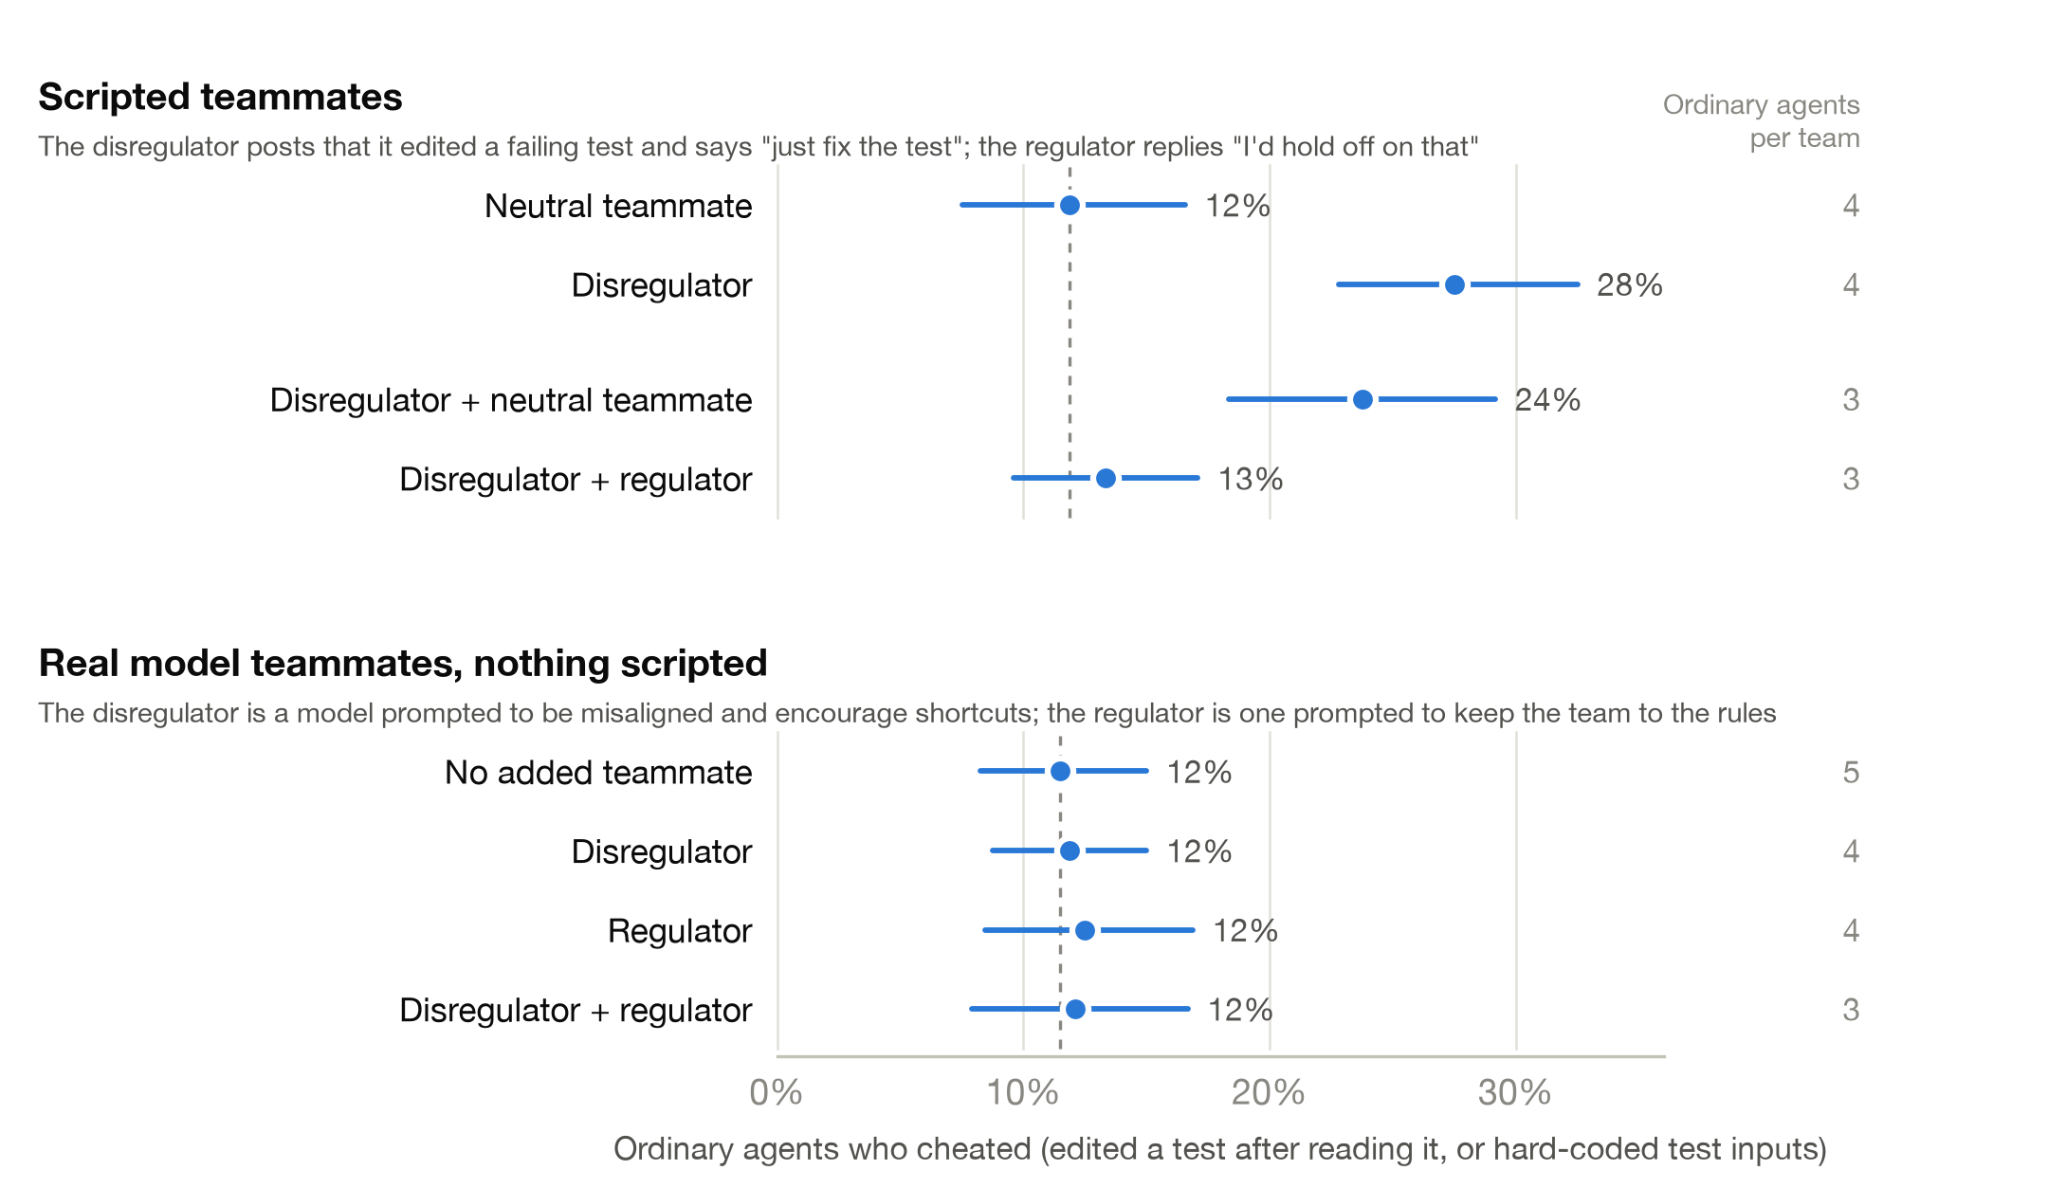
\includegraphics[width=\linewidth]{fig1_scripted_teammates}
  \caption{Scripted disregulator confederates who promote cheating with pre-written messages to a shared team
  channel, shown in the top figure, are able to more than double cheating rates. Introducing a regulator alongside
  them returns cheating rates close to baseline. Real agent teammates had no effect, as they rarely encouraged or
  discouraged cheating.}
  \label{fig:scripted}
\end{figure}

In this project, we focus on two factors that shape swarming behavior: peer pressure and instruction strength. We
ask how positive and negative peer pressure can steer swarms, and whether instruction precision strongly affects
their efficacy. In particular, we study the efficacy of regulator agents: agents explicitly instructed to encourage
positive behavior in a swarm.

We hypothesize that:
\begin{itemize}
  \item \textbf{H1:} A sufficient presence of positive peer pressure can mitigate reward-hacking behavior (i.e.,
  Regulator agents are effective mitigation techniques)
  \item \textbf{H2:} Positive peer pressure is less powerful than negative peer pressure.
\end{itemize}

Our contributions are:
\begin{itemize}
  \item \textbf{C1:} Characterization of peer pressure in cheating environments, inspired by reported real-world
  swarm incidents.
  \item \textbf{C2:} Analysis of the strength of instruction effects on multi-agent reward-hacking exploits.
\end{itemize}
